% Results and Discussion section.
% \ref{sec:results} is the target of the validation sentence in the methods section.
% Filter thresholds below are taken verbatim from the downstream-filter notebook.

\begin{figure*}[!b]
  \centering
  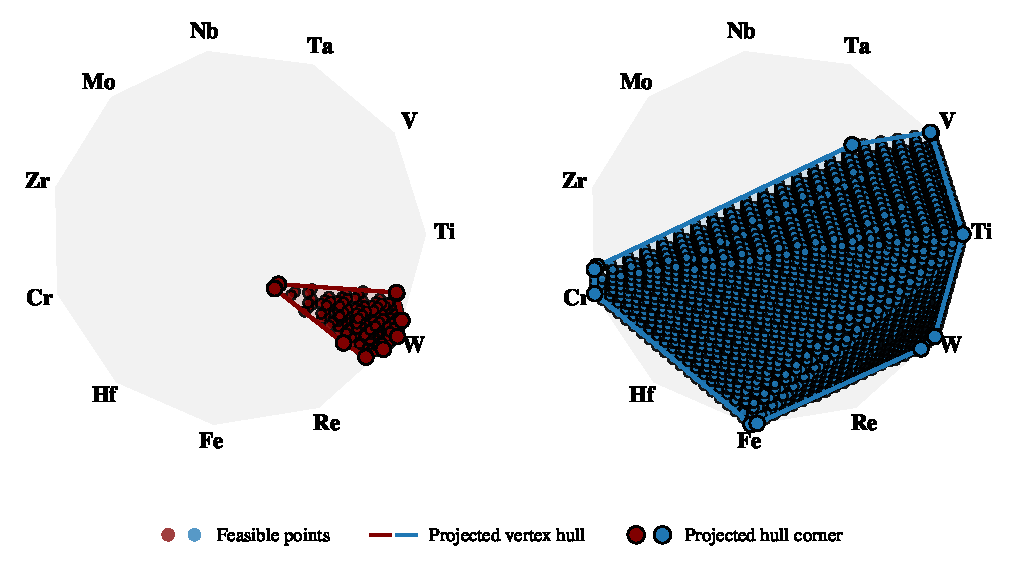
\includegraphics[width=0.90\textwidth]{figures/LP-FLARE-polytope-5at-10x.pdf}
  \caption{Activation-feasible compositions from the LP screen, projected onto the
eleven-element composition simplex. The left panel shows the \(10\times\)W
feasible region, and the right panel the \(10\times\)EUROFER97 region, with feasible
compositions as points and the projected vertex hull outlined.}
  \label{fig:polytope}
\end{figure*}

\section{Results and Discussion}
\label{sec:results}

\subsection{Feasible Space and Neutronic Screening}
\label{subsec:feasible}
Sampling of an eleven-element Cr-Fe-Hf-Mo-Nb-Re-Ta-Ti-V-W-Zr alloy
space on a \(5\)~at.\% grid yields \(30{,}045{,}015\) candidate
compositions, and evaluating every candidate individually at this scale
is costly. Since the activation responses are linear
in composition, the feasible region is instead constructed directly as a
polytope from the constraints, and the grid compositions lying inside it are
enumerated, producing \(210\) feasible compositions under the
\(10\times\)W reference and \(61{,}297\) under \(10\times\)EUROFER97.
The two feasible regions are shown projected onto the composition simplex in Fig.\ref{fig:polytope}. The two orders of magnitude
difference between the two sets reflects the baseline responses of the
references, since ten times a lower baseline is the tighter bound.
Although all eleven elements were free to vary, only Ti, V, Zr, Cr, Fe, Re, and W occur in the feasible compositions of either screen. The remaining four elements, Ta, Nb, Mo, and Hf, are excluded entirely by the activation criteria rather than by any prior restriction. By construction, every surviving composition remains within a factor
of ten of its reference material for all activation responses under the
irradiation conditions of Table~\ref{tab:ind_variables}, and this bound is retained through
the subsequent property screens.

The constraint-first approach was verified against a brute-force FLARE
evaluation of the full grid, which returned the same feasible compositions
under each reference, with every response agreeing to numerical precision.
The two approaches reach this result with different effort. The polytope
enumeration, which touches only the feasible set, completed in
\textcolor{red}{\texttt{Insert Runtime}}, while brute force evaluates every
grid candidate explicitly and becomes rapidly more expensive as the grid
grows. The deviation factor remains a tunable setting, and stricter or looser
values than the tenfold tolerance used here would contract or expand the
space accordingly, since the constraint bounds scale directly with it.


\subsection{Property Screening and Feasible Subgraphs}
\label{subsec:subgraphs}

For subgraph selection, the activation-feasible alloys identified in
Section~\ref{subsec:feasible} were evaluated with CALPHAD for phase stability and thermal
conductivity. The alloys from the two screens were merged into a single set, and
the \(204\) duplicated compositions were removed, leaving \(61{,}298\)
unique compositions. A candidate alloy is retained when its BCC phase fraction is at least $0.98$ at $500$, $600$, and $650\,^{\circ}\mathrm{C}$, keeping it single-phase, and when its room-temperature thermal conductivity exceeds $16~\mathrm{W/(m\cdot K)}$ for efficient heat transport. Applying both criteria together leaves $700$ compositions, representing $1.1\%$ of the $61{,}298$ candidate alloys, concentrated in the \ch{W-V-Cr-Fe} region of the simplex.


The connectivity of these (700) compositions after applying the two constraints is shown in Fig.~\ref{fig:clusters}, forming three disconnected subgraphs. Subgraph~1 contains (686) compositions, about (98\%) of the survivors, and forms a connected region spanning the \ch{W-V-Cr-Fe} band from the tungsten-rich corner to the vanadium- and titanium-rich region. Subgraphs~2 and~3 are small isolated islands of eight and six compositions, feasible in every screened property yet unreachable from Subgraph~1. A path within a subgraph moves between compositions in small steps without leaving the feasible set, whereas crossing between subgraphs would require passing through infeasible compositions. Subgraph~1, offering the largest contiguous space for a graded transition, is therefore carried forward as the design region for the graded alloy.


\begin{figure}[H]
  \centering
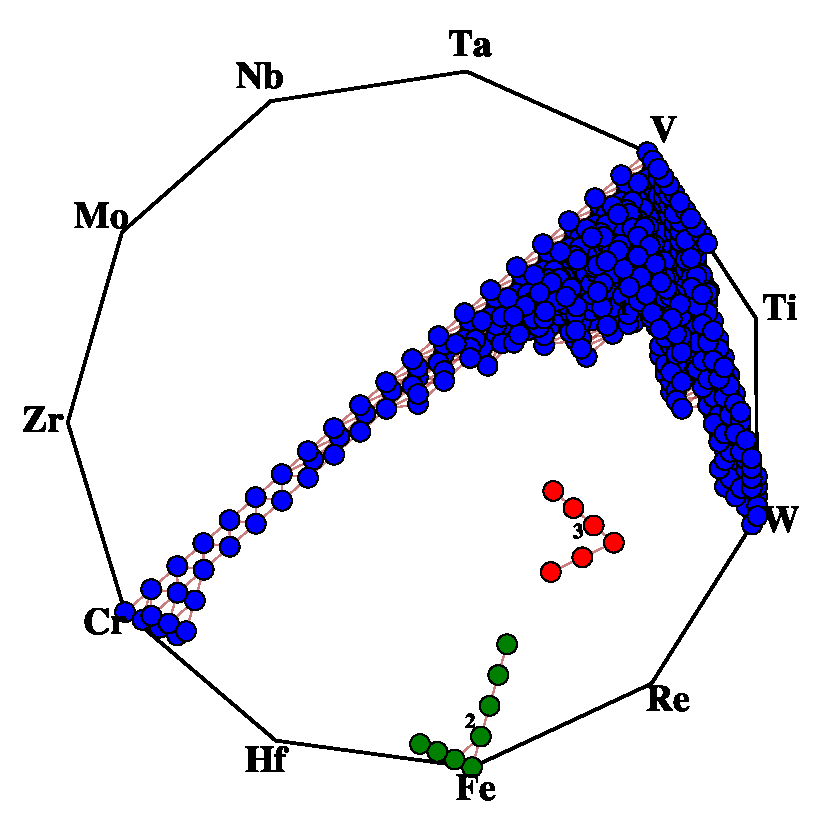
\includegraphics[width=0.75\linewidth]{manuscript/figures/LP_FLARE_nim_fig1_all_subgraphs.pdf}
 \caption{Feasible compositions in the eleven-element design space after neutronics,
phase, and thermal-conductivity screening.}
  \label{fig:clusters}
\end{figure}

%The combined feasible set, comprising the survivors of both the \(10\times\)W and\(10\times\)EUROFER97 screens, is next evaluated for its thermodynamic and thermophysical properties by CALPHAD and subjected to fusion-relevant property constraints in two stages. The \(204\) compositions feasible under both references were equilibrated in both screening passes and thus serve as replicate calculations: \(199\) agree to within \(1\)~K in solidus, mutually validating the CALPHAD inputs, while the remaining five, tungsten-rich compositions bearing Fe and Re, disagree beyond tolerance and are excluded as non-converged equilibria, leaving \(61{,}298\) unique compositions for property screening. The first stage applies two universal requirements, a stable single-phase BCC structure, taken as a maximum BCC mole fraction of at least \(0.98\) at \(500\), \(600\), and \(650\,^{\circ}\mathrm{C}\), and a room-temperature thermal conductivity above \(16\)~W/(m\,K), selecting for phase stability across the operating range and for adequate heat removal.

%\begin{figure}[H]
  %\centering
%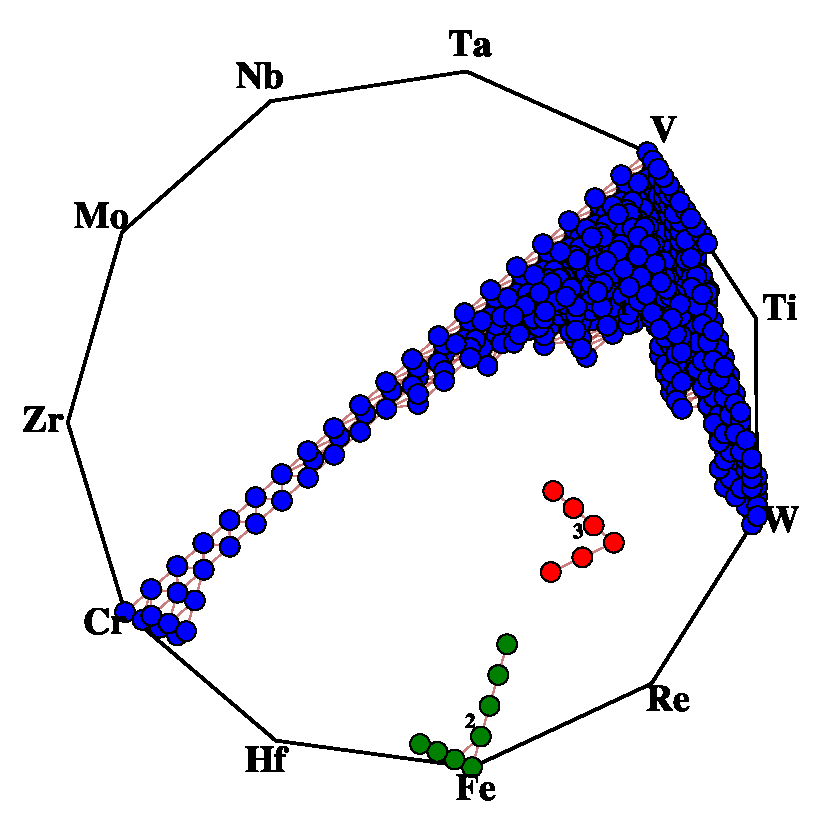
\includegraphics[width=0.75\linewidth]{manuscript/figures/LP_FLARE_nim_fig1_all_subgraphs.pdf}
 %\caption{Feasible compositions in the eleven-element design space after neutronics,
%CALPHAD, and thermal-conductivity screening. Subgraph~1 (blue) represents the largest connected set, suitable for FGM development.}
  %\label{fig:clusters}
%\end{figure}

%To group the surviving compositions, those passing the BCC and conductivity filters are connected into a traversal graph on the composition lattice: each feasible composition is a node, and two nodes share an edge when they differ by a single \(5\)~at.\% exchange between two elements, following the simplex-lattice adjacency of NIMPLEX~\cite{nimplex}. The connected components of this graph are the feasible subgraphs (Figure~\ref{fig:clusters}). This grouping has a direct physical meaning, since a path within a single component moves between compositions in small steps without leaving the feasible set, whereas crossing between components would require passing through infeasible compositions~\cite{nimplex}. Of the \(700\) compositions surviving both filters, three components result: a large subgraph of \(686\) compositions spanning the \ch{W-V-Cr-Fe} band and two much smaller, genuinely isolated islands of \(8\) and \(6\) compositions, feasible in every property yet unreachable from the main region by any single \(5\)~at.\% step. The largest, being the most connected region of the feasible set, is the natural candidate for a graded plasma-facing-to-structural material and is carried forward.



\subsection{Plasma-Facing and Structural Alloy Classification}

The \(686\) compositions of Subgraph~1 were classified according to
two design targets, a solidus temperature above
\(2200\,^{\circ}\mathrm{C}\) for high-temperature capability and a Pugh
ratio of \(2.6\) for intrinsic ductility. Compositions meeting the solidus requirement are designated Alloy~A
and are the plasma-facing material (PFM) candidates, and those meeting the
ductility requirement are designated Alloy~B, the structural candidates.
Compositions meeting both requirements are designated Alloy~AB, and these
satisfy the demands of both sides and serve as a bridge between the
plasma-facing and structural regions. The remaining compositions, which meet
neither requirement, are designated Intermediate and are not considered in
the terminal selection, although they remain part of the traversable design
region. Of these, \(148\) qualify as
Alloy~A, \(353\) as Alloy~B, \(18\) as Alloy~AB, and \(167\) are
Intermediate. Their distribution across the simplex is shown in
Figure~\ref{fig:categories}, where Alloy~A clusters in the tungsten-rich
corner and Alloy~B in the vanadium-rich region. The
two-property classification thus identifies the plasma-facing and structural
materials within the design region, with the small Alloy~AB set lying
between them and reconciling high-temperature capability with intrinsic
ductility.

\begin{figure}[H]
  \centering
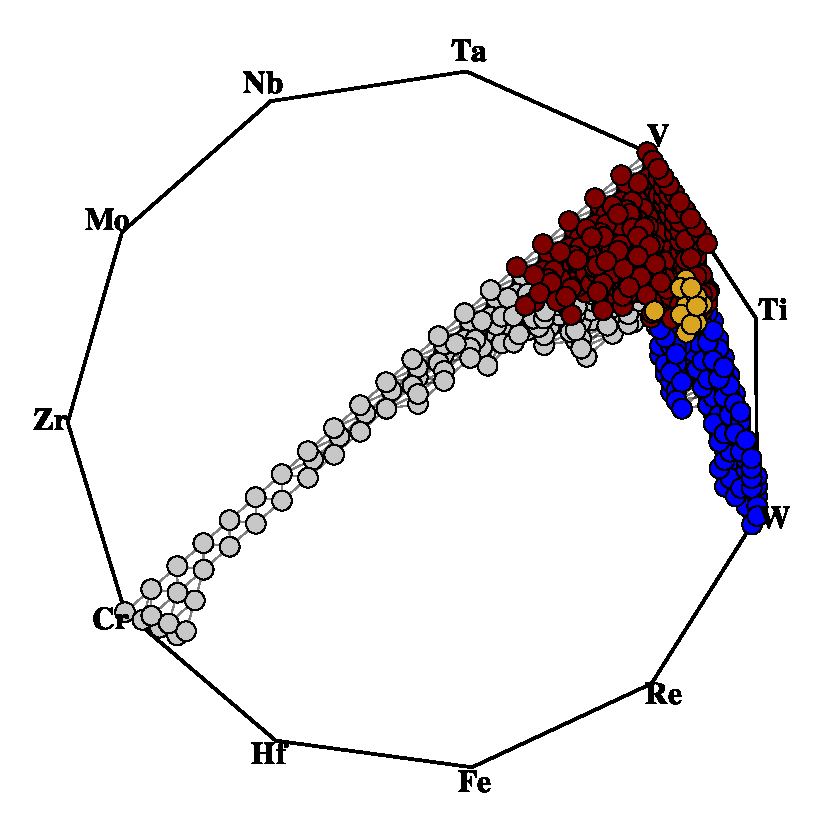
\includegraphics[width=0.75\linewidth]{figures/LP_FLARE_nim_fig2_subgraph1_categories.pdf}
\caption{Candidate categories of Subgraph~1 on the composition simplex,
with Alloy~A in blue, Alloy~B in maroon, Alloy~AB in goldenrod, and
Intermediate in grey.}
  \label{fig:categories}
\end{figure}

Fig.~\ref{fig:properties} maps the two classification properties
over Subgraph~1, with the Pugh ratio in panel~(a) and the solidus
temperature in panel~(b). The two maps display opposite gradients. The Pugh
ratio increases from the tungsten-rich corner toward the vanadium-rich compositions, while the solidus temperature peaks in the
tungsten-rich corner and falls in the direction the ductility rises, so that
the two properties are strongly anticorrelated across the subgraph. The
subgraph therefore spans a continuous trade-off between high-temperature
capability and ductility, and the maps locate where each design target is
met, with the plasma-facing candidates at one end and the structural
candidates at the other. The graded-path design of the next section is built on this classified region.

\label{subsec:classification}
\begin{figure*}[b]
  \centering
  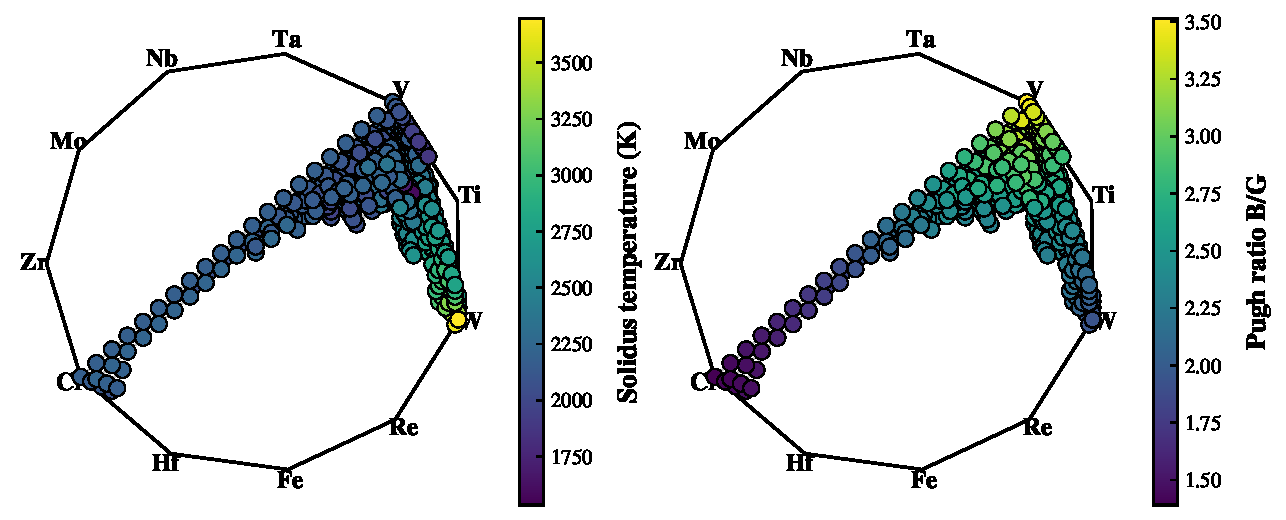
\includegraphics[width=0.80\textwidth]{figures/LP_FLARE_nim_fig3_subgraph1_properties.pdf}
  \caption{CALPHAD properties across the largest connected subgraph, projected
  onto the composition simplex: (a) Pugh ratio (\(B/G\)) and (b) solidus
  temperature.}
  \label{fig:properties}
\end{figure*}


\subsection{Doubly-Monotonic Path Planning}
\label{subsec:path}
The design question is whether the two regions identified in
Section~\ref{subsec:classification} can be joined by a compositional
gradient whose properties evolve in one direction only, so that no interior
layer of the graded wall is hotter-melting than the layer in front of it or
less ductile than the layer behind it. This is posed as a path problem on the traversal graph of
Subgraph~1, with terminals restricted to deployable multi-component alloys
of at least three constituents and no single element above \(90\)~at.\%.
Without this restriction, the property extrema are the pure elements, and the
design degenerates to a trivial W\(\to\)V elemental gradient anchored by
non-deployable terminals. Within the deployable pools (\(147\) plasma-facing
and \(342\) structural candidates), the plasma-facing terminal is taken as
the maximum-solidus composition among the Alloy~A and AB candidates and the
structural terminal as the maximum-Pugh composition among the Alloy~B and AB
candidates. Monotonicity is enforced as a hard constraint by removing from the
traversal graph every directed edge that raises the solidus or lowers the
Pugh ratio, after which Dijkstra's algorithm returns the exact shortest path
on what remains. The search objective is unweighted path
length, so the formulation contains no tuning parameters, in contrast to
penalized cost-function approaches in which monotonicity is promoted through a
weight that must be selected~\cite{kirk2021monotonic}.


The resulting terminals are V\(_{5}\)Re\(_{5}\)W\(_{90}\) (solidus
\(3449\)~K) for the plasma-facing role and Ti\(_{5}\)V\(_{90}\)Re\(_{5}\)
(Pugh ratio \(3.34\)) for the structural role. A strict doubly-monotonic path
between them exists, consisting of \(19\) alloys connected by \(18\) steps of
a single \(5\)~at.\% exchange each, along which the solidus never rises and
the Pugh ratio never falls from one step to the next, verified independently
by per-step assertion and by a loss-of-invariance metric of zero for both
properties (Figures~\ref{fig:path} and~\ref{fig:path-profiles}). At each
step, \(5\)~at.\% of one element is exchanged for another, the smallest
possible move between neighboring compositions on the design grid. Every
intermediate composition on the path satisfies the activation,
phase-stability, and conductivity screens by construction. Eighteen
steps is also the minimum conceivable for this terminal pair, since
the tungsten content alone must change by eighteen lattice units, so the
monotonicity requirement is achieved at zero cost in path length. The pruned
formulation, in which only \(2{,}030\) of the \(7{,}348\) directed
transitions in Subgraph~1 survive, guarantees this by construction, as any
shortest path on the pruned graph is monotone.

\begin{figure}[H]
  \centering
  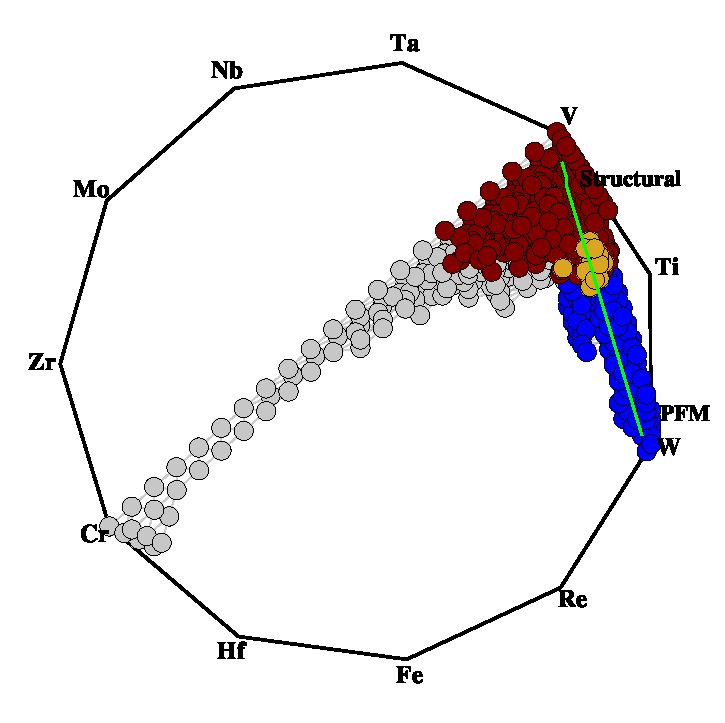
\includegraphics[width=0.8\linewidth]{figures/LP_FLARE_nim_fig6_graded_path.pdf}
  \caption{The shortest doubly-monotonic path (green) across the
classified compositions of Subgraph~1, from the PFM terminal to the
structural terminal on the composition simplex.
Node colors follow Figure~\ref{fig:categories}.}
  \label{fig:path}
\end{figure}

Fig.~\ref{fig:path-profiles} shows the property evolution along
this route. The solidus falls from \(3449\) to
\(2195\)~K and the Pugh ratio rises from \(2.00\) to \(3.34\), with the
largest solidus drops concentrated in the tungsten-rich early steps and the
largest ductility gains toward the vanadium-rich end. The two curves cross
their respective category thresholds within the Alloy~AB window, at steps 10 to 12 of the path.

\begin{figure}[H]
  \centering
  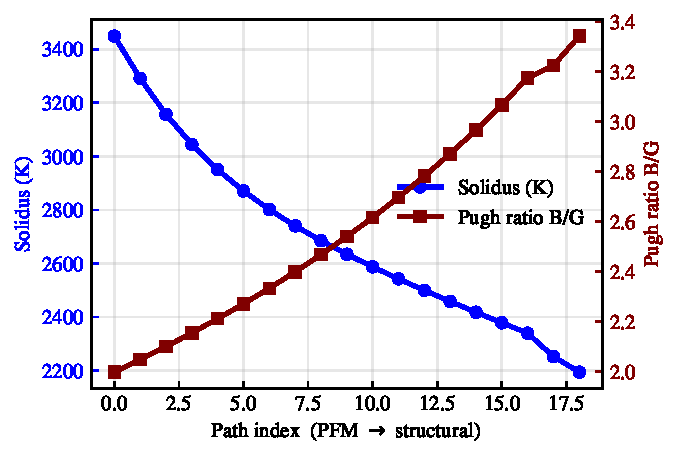
\includegraphics[width=1\linewidth]{figures/LP_FLARE_nim_fig7_path_property_profile.pdf}
  \caption{Solidus temperature and Pugh ratio along the path, from the
plasma-facing terminal (index~0) to the structural terminal (index~18). The
solidus is non-increasing and the Pugh ratio non-decreasing at every step.}
  \label{fig:path-profiles}
\end{figure}

The \(18\) Alloy~AB compositions prove structurally essential to this result.
A connectivity test on the pruned graph shows that no doubly-monotonic
route exists between the terminals when these compositions are removed, as
every admissible route from the plasma-facing candidates to the structural
candidates is forced through the dual-criteria class, and the optimal path
traverses three of its eighteen members. The overlap of the two property criteria is
therefore not incidental but constitutes the sole monotone gateway between
the plasma-facing and structural categories. To our knowledge, enforcing monotonicity in two
opposing properties simultaneously has not been reported in the
compositionally graded alloy path-planning literature, which has treated
monotonicity in a single property~\cite{kirk2021monotonic}. The
complete path is given in Table~\ref{tab:path}, traversing the Alloy~A, AB,
and B categories in sequence.

\begin{table*}[!t]
\centering
\caption{The shortest doubly-monotonic graded path: nineteen alloys connected by
eighteen steps of a single 5~at.\% exchange each, from the plasma-facing terminal
(index~0) to the structural terminal (index~18). The solidus is non-increasing
and the Pugh ratio non-decreasing at every step; the three Alloy~AB compositions
(indices 10-12) constitute the monotone gateway between the two categories.}
\label{tab:path}
\begin{tabular}{clllcc}
\toprule
Index & Composition (at.\%) & Step & Solidus (K) & Pugh $B/G$ & Category \\
\midrule
0 & V$_{5}$Re$_{5}$W$_{90}$ & -- & 3449 & 2.00 & A \\
1 & V$_{10}$Re$_{5}$W$_{85}$ & W\,$-5$, V\,$+5$ & 3292 & 2.05 & A \\
2 & V$_{15}$Re$_{5}$W$_{80}$ & W\,$-5$, V\,$+5$ & 3157 & 2.10 & A \\
3 & V$_{20}$Re$_{5}$W$_{75}$ & W\,$-5$, V\,$+5$ & 3045 & 2.15 & A \\
4 & V$_{25}$Re$_{5}$W$_{70}$ & W\,$-5$, V\,$+5$ & 2951 & 2.21 & A \\
5 & V$_{30}$Re$_{5}$W$_{65}$ & W\,$-5$, V\,$+5$ & 2871 & 2.27 & A \\
6 & V$_{35}$Re$_{5}$W$_{60}$ & W\,$-5$, V\,$+5$ & 2802 & 2.33 & A \\
7 & V$_{40}$Re$_{5}$W$_{55}$ & W\,$-5$, V\,$+5$ & 2741 & 2.40 & A \\
8 & V$_{45}$Re$_{5}$W$_{50}$ & W\,$-5$, V\,$+5$ & 2686 & 2.47 & A \\
9 & V$_{50}$Re$_{5}$W$_{45}$ & W\,$-5$, V\,$+5$ & 2635 & 2.54 & A \\
10 & V$_{55}$Re$_{5}$W$_{40}$ & W\,$-5$, V\,$+5$ & 2588 & 2.62 & AB \\
11 & V$_{60}$Re$_{5}$W$_{35}$ & W\,$-5$, V\,$+5$ & 2543 & 2.70 & AB \\
12 & V$_{65}$Re$_{5}$W$_{30}$ & W\,$-5$, V\,$+5$ & 2500 & 2.78 & AB \\
13 & V$_{70}$Re$_{5}$W$_{25}$ & W\,$-5$, V\,$+5$ & 2459 & 2.87 & B \\
14 & V$_{75}$Re$_{5}$W$_{20}$ & W\,$-5$, V\,$+5$ & 2418 & 2.97 & B \\
15 & V$_{80}$Re$_{5}$W$_{15}$ & W\,$-5$, V\,$+5$ & 2379 & 3.07 & B \\
16 & V$_{85}$Re$_{5}$W$_{10}$ & W\,$-5$, V\,$+5$ & 2340 & 3.18 & B \\
17 & Ti$_{5}$V$_{85}$Re$_{5}$W$_{5}$ & W\,$-5$, Ti\,$+5$ & 2253 & 3.23 & B \\
18 & Ti$_{5}$V$_{90}$Re$_{5}$ & W\,$-5$, V\,$+5$ & 2195 & 3.34 & B \\
\bottomrule
\end{tabular}
\end{table*}



Fig.~\ref{fig:path-composition} shows the compositional simplicity
of the path. Tungsten declines and vanadium rises together across sixteen
consecutive exchanges, rhenium remains a constant \(5\)~at.\% from terminal
to terminal, and titanium enters only in the final two layers as the tungsten
is exhausted. Although the path was searched
in an eleven-element space, it engages only four elements, and at no point do
more than four coexist. In practical terms, the entire gradient can be
deposited from two varying feed streams against a constant rhenium addition,
with a single titanium introduction near the structural end


\begin{figure}[H]
  \centering
  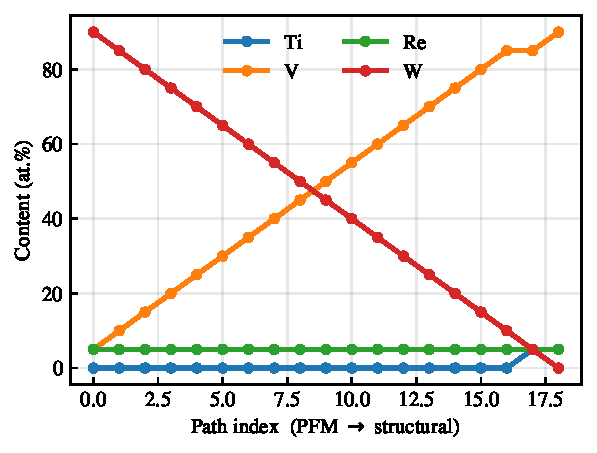
\includegraphics[width=0.9\linewidth]{figures/LP_FLARE_nim_fig8_path_composition_profile.pdf}
  \caption{Elemental composition along the path: a tungsten-vanadium
substitutional gradient at constant 5~at.\% Re, with Ti introduced in the
final two layers as W is exhausted. Each step changes exactly one element pair
by 5~at.\%.}
  \label{fig:path-composition}
\end{figure}


\subsection{ELM Assessment of the Graded Design}
\label{subsec:elm}

As a final assessment, the graded design is evaluated against transient
edge-localized-mode (ELM) heat loading, the surface requirement that the
equilibrium screens do not address. The assessment was carried out over all
\(686\) compositions of Subgraph~1, so that the melting capability of the
entire classified region is established rather than that of the path alone.
For each composition, the peak surface temperature during an ELM pulse was
computed from its CALPHAD-derived thermal properties
(Section~\ref{subsec:elm-methods}), and the ELM melting margin was defined
as the alloy solidus minus this peak temperature, so that a positive margin
means the surface stays below melting.

Fig.~\ref{fig:elm} shows the margin across the classified region. It
ranges from \(-4140\) to \(+2229\)~K with a mean of \(-806\)~K, and \(114\)
of the \(686\) compositions (\(17\%\)) remain positive. The margin
correlates strongly with tungsten content, the passing compositions
averaging \(57\)~at.\% W against \(12\)~at.\% W for those that fail, since
tungsten raises the solidus that the surface temperature is measured
against. The ELM-resistant set is not limited to near-pure
tungsten. Tungsten alloyed with Ti, V, and Re retains a positive margin, and
a small group of Cr-rich compositions also passes, eight of the thirty-one
with at least \(50\)~at.\% Cr, so several compositional routes to ELM
resistance exist within the region. The pass/fail boundary is sharp, with
\(76\) compositions lying within \(\pm200\)~K of zero margin.

\begin{figure*}[!t]
  \centering
  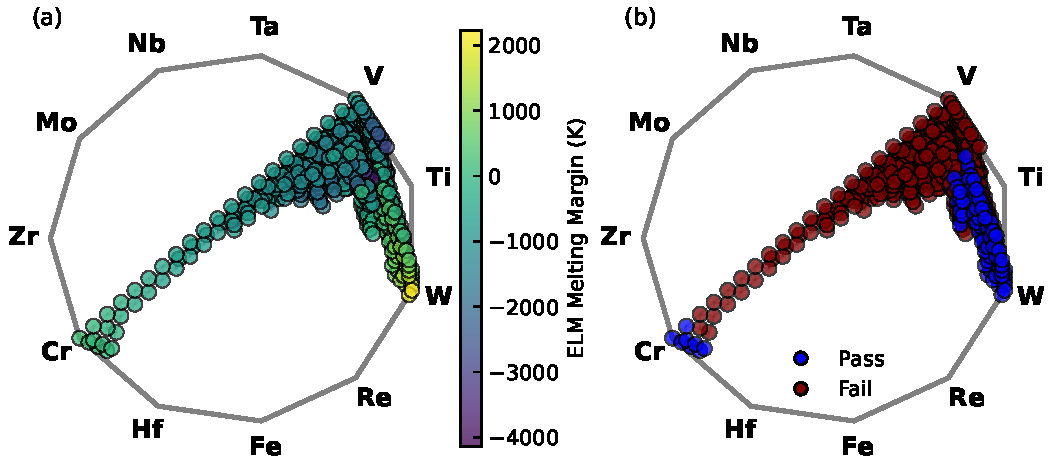
\includegraphics[width=0.80\textwidth]{figures/LP-FLARE-ELM-margin-panels.pdf}
  \caption{ELM assessment across the largest connected subgraph, projected
onto the composition simplex: (a) ELM melting margin and (b) the resulting
pass/fail classification, with blue marking compositions of positive margin
(pass) and maroon those of negative margin (fail).}
  \label{fig:elm}
\end{figure*}

The graded path passes this test exactly where it must. Its plasma-facing
terminal, V\(_{5}\)Re\(_{5}\)W\(_{90}\), carries a margin of \(+1650\)~K,
placing it comfortably within the ELM-resistant set, and the margin
decreases smoothly along the path, remaining positive through the first
twelve layers, the entire Alloy~A segment and two of the three gateway
compositions before crossing zero at the transition into the structural
category. The ELM-resistant extent of the gradient therefore coincides with
its plasma-facing function, as the layers that face the plasma withstand the
transient while the structural layers behind them, shielded from surface
loading, are not required to. The ELM assessment thus adds a third,
independent line of evidence that converges with the activation and
mechanical screens on the same separation of plasma-facing and structural
materials, now traced layer by layer along the designed gradient.